\documentclass[../../main.tex]{subfiles}

% 

\begin{document}
\chapter{Dopplerov jav v spektroskopii}

\section{Teória okolo Dopplerovho javu}

\subsection{Klasický Dopplerov jav}

Dopplerov jav (alebo Dopplerov posun) je jav pri ktorom dochádza k zmene frekvencie a vlnovej dĺžky vlny pre pozorovateľa, ktorý sa pohybuje vzhľadom na zdroj vlnenia. Tento efekt je pomenovaný po rakúskom fyzikovi Christiánovi Dopplerovi\footnote{ktorý pracoval ako profesor v Prahe a neskôr aj v Banskej Štiavnici}, ktorý ho opísal v roku 1842.

Doppler prvýkrát spomenul tento jav v jednej zo svojich prác\footnote{"Über das farbige Licht der Doppelsterne und einiger anderer Gestirne des Himmels"} a o tri roky neskôr jeho hypotézu úspešne otestoval na zvukových vlnách Buys Ballot. Nezávisle od Dopplera objavil Hippolyte Fizeau tento jav pre elektromagnetické vlny v roku 1848, takže vo Francúzsku bol chvíľu jav označovaný ako Doppler-Fizeauov jav, no vo svete sa tento názov neujal, keďže Fizeau bol za Dopplerom 6 rokov pozadu.

\begin{figure}[h]
\centering
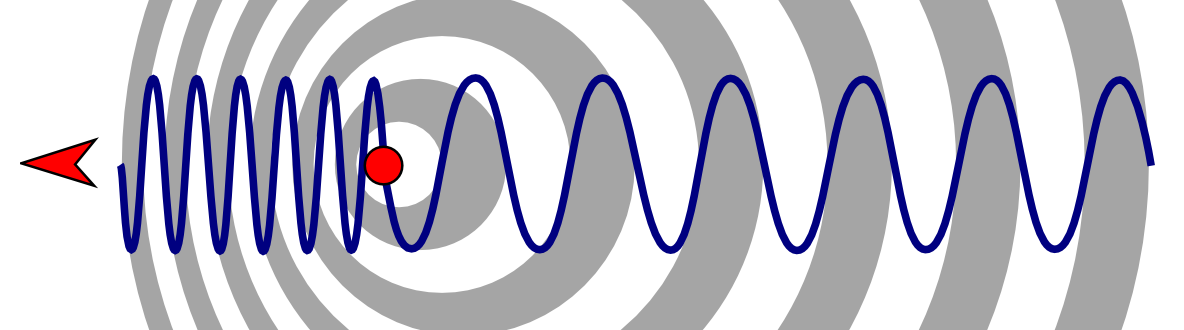
\includegraphics[width=\textwidth]{js9-doppler.png}
\caption{Dopplerov jav}
\label{js9:img:doppler}
\end{figure}


\paragraph{Odvodenie:} Predstavme si, že máme zdroj, ktorý sa pohybuje smerom k pozorovateľovi rýchlosťou $v_z$. Takýto zdroj vyžiari vlnu s frekvenciou $f_0$ a vlnovou dĺžkou $\lambda_0$. Začiatok vlny je vyžiarený v čase $t_0=0$ a koniec vlny je vyžiarený v čase $t'_0=\frac{\lambda_0}{c}=\frac{1}{f_0}$. Ďalej uvažujme, že v čase 0 bola vzdialenosť medzi zdrojom a pozorovateľom $d$ a pozorovateľ sa pohyboval rýchlosťou $v_p$ smerom ku zdroju. Začiatok vlny preto dojde k pozorovateľovi v čase $t_1$, pre ktorý platí vzťah
\begin{equation}
d=t_1 c+t_1 v_p
\end{equation}

Koniec vlny dorazí k pozorovateľovi v čase $t'_1$, pre ktorý platí rovnica
\begin{equation}
d-t'_0 (v_z+v_p)=(t'_1-t'_0)(c+v_p)
\end{equation}
Rozdielom časov dostaneme periódu vlnenia, ktorá je prevrátenou hodnotou frekvencie.
\begin{equation}
T=t'_1-t_1=\dfrac{d-t'_0v_z+t'_0c}{c+v_p}-\dfrac{d}{c+v_p}=\dfrac{1}{f_0}\dfrac{c-v_z}{c+v_p}
\end{equation}

V klasickej fyzike, kedy rýchlosť zdroja a pozorovateľa vzhľadom na okolie sú menšie ako rýchlosť svetla, platí teda vzťah medzi pozorovanou frekvenciou $f$ a emitovanou frekvenciou $f_0$ vzťah
\begin{equation}
f=\left(\dfrac{c+v_p}{c-v_z}\right) f_0
\end{equation}
kde $c$ je rýchlosť vĺn, $v_p$ je rýchlosť pozorovateľa (ktorá je kladná, keď sa pozorovateľ pohybuje k zdroju a naopak) a $v_z$ je rýchlosť zdroja (ktorá je kladná, keď sa zdroj pohybuje k pozorovateľovi a naopak).

\subsection{Relativistický Dopplerov jav}

V prípade elektromagnetického žiarenia, ktoré je emitované zdrojom pohybujúcim sa rýchlosťou blízkou rýchlosti svetla\footnote{alebo pozorovateľom pohybujúcim sa takto veľkou rýchlosťou} je potrebné započítať efekty dilatácie času.

Odvodenie je podobné tomu klasickému s tým rozdielom, že v tomto prípade nezáleží na tom, či sa pohybuje zdroj alebo pozorovateľ, dôležitá je iba celková vzájomná rýchlosť $v$. Pridáme preto relativistické efekty a pre frekvenciu dostaneme
\begin{equation}
f=\gamma \left( 1-\dfrac{v}{c}\right)f_0=\gamma(1-\beta)f_0=f_0\sqrt{\dfrac{1-\beta}{1+\beta}}=f_0\sqrt{\dfrac{1-\frac{v}{c}}{1+\frac{v}{c}}}
\end{equation}

\section{Dopplerovské rozšírenie}

Dopplerovské rozšírenie (angl. Doppler broadening) je rozšírenie spektrálnych čiar v dôsledku Dopplerovho javu spôsobené nemonofrekvenčným rozdelením rýchlostí atómov v molekulách. Rôzne rýchlosti emitujúcich častíc spôsobujú rôzny Dopplerov posun, a to vo výsledku spôsobuje rozšírenie. Výlsedný profil je známy ako Dopplerovský profil. Časť Dopplerovského rozšírenia, ktorá je spôsobená tepelným pohybom častíc nazývame tepelné Dopplerovské rozšírenie. V takom prípade rozširenie závisí iba na frekvencii spektrálnej čiary, hmotnosti emitujúcich častíc a ich teplote.

Dopplerovské rozšírenie je popísané pravdepodobnostným rozdelením
\begin{equation}
P_f(f)\mathrm{d}f=\sqrt{\dfrac{mc^2}{2\pi kTf_0^2}} \exp\left(-\dfrac{mc^2(f-f_0)^2}{2kTf_0^2}\right)\mathrm{d}f,
\end{equation}
kde $m$ je hmotnosť emitujúcej častice, $f$ je pozorovaná frekvencia a $f_0$ je pokojová frekvencia. Toto rozdelenie vzniklo jednoduchým vyjadrením rýchlosti z Dopplerovho javu ako $v=c(\frac{f}{f_0}-1)$ a dosadením do klasického Maxwellovho rozdelenia.

\section{Nasýtená absorpčná spektroskopia}

Aby sme dokázali určiť skutočnú frekvenciu atómových prechodov bez potreby schladenia vzorky na veľmi nízke teploty, využívame \textit{nasýtenú absorpčnú spektroskopiu}\footnote{angl. saturation absorption spectroscopy}, ktorá je tiež známa pod pojmom antidopplerovská spektroskopia\footnote{angl. Doppler-free spectroscopy}. Pri tomto procese ožarujeme atómový plyn laserom s relatívne vysokou frekvenciou. Tento lúč nazývame \textit{pumpovací}\footnote{angl. pump beam}. Okrem neho je plyn ožarovaný aj ďalším slabším lúčom s rovnakou frekvenciou. Ten nazývame \textit{snímací} lúč\footnote{angl. probe beam}. Snímací lúč je rozdelený na polovice, jedna polovica prejde plynom a zaznamená sa, druhá polovica ide v protismere pumpovacieho lúča a následne sa tiež zaznamená. Absorpcia snímacieho lúča je zaznamenávaná na fotodiódu pre rôzne frekvencie lúčov.

\begin{figure}[h]
\centering
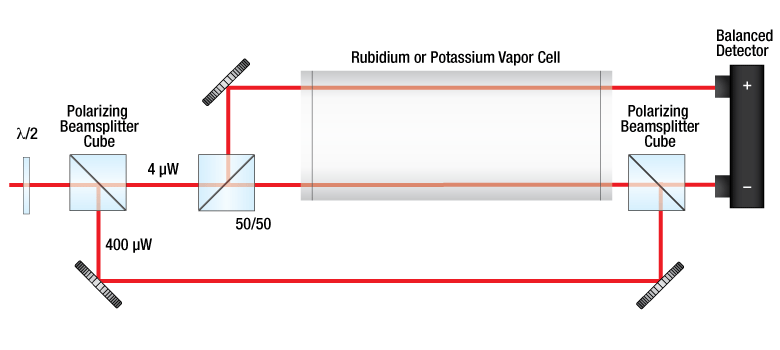
\includegraphics[width=\textwidth]{js9-sasschema.png}
\caption{Schéma nasýtenej absorpčnej spektroskopie.}
\label{js9:img:sasschema}
\end{figure}

Napriek tomu, že lúče majú rovnakú frekvenciu, zasahujú rôzne atómy kvôli tepelnému pohybu. V prípade, že frekvencia lúčov je posunutá k červenej farbe (\textit{red-detuned}) vzhľadom na frekvenciu prechodu atómu, znamená to, že pumpovací lúč bude absorbovaný atómom pohybujúcim sa k zdroju lúčov a snímací lúč bude absorbovaný atómom pohybujúcim sa od zdroja. Ak je frekvencia posunutá k modrej farbe (\textit{blue-detuned}), nastane presný opak.

V prípade, že má laser rezonančnú frekvenciu, oba lúče zasiahnu rovnaké atómy, a to tie, ktoré sa pohybujú kolmo na smer lúčov. V prípade, že uvažujeme aproximáciu atómových prechodov ako systém s dvomi stavmi, silný pumpovací lúč spôsobí, že mnoho atómov bude v excitovanom stave. Keď je počet atómov v základnom a excitovanom stave približne rovnaký, prechod je nazývaný nasýteným. Keď fotón zo snímacieho lúča prejde plynom, je veľká šanca, že zasiahne atóm, ktorý je excitovaný a dôjde k stimulovanej emisii. Kvôli tomu pri postupnom menení frekvencie lúčov v okolí rezonancie vznikne malá jama v každom z atómových prechodov. Čím je pumpovací lúč silnejší, tým užšiu a hlbšiu jamku dostaneme. Pri perfektných podmienkach môže jamka dosiahnuť tvar prirodzenej šírky prechodu.
\vspace{1cm}

\begin{figure}[h!]
\centering
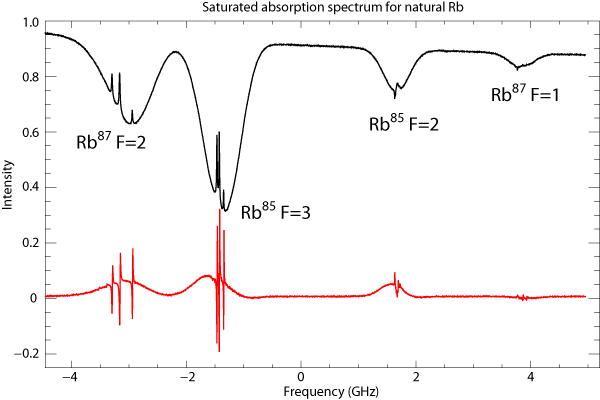
\includegraphics[width=0.8\textwidth]{js9-sasspectrum.png}
\caption{Čiernou farbou je znázornené spektrum na výstupe nasýtenej absorpčnej spektroskopie a červenou je spektrum po odčítaní spektra priameho prechodu.}
\label{js9:img:sasspectrum}
\end{figure}

\section{Využitie metód založených na Dopplerovom posune}

Dopplerov jav sa využíva pri určovaní pravdepodobnosti prechodu z dôb života. Pri jadrovej reakcii vznikne excitované jadro v tenkom terčíku. Toto jadro opustí terčík s určitou rýchlosťou, ktorá je daná zo zákona zachovania hybnosti ako
\begin{equation}
v=\dfrac{v_am_a}{m_a+M_A}=c\dfrac{\sqrt{2m_ac^2E_{kin,a}}}{(m_a+M_A)c^2},
\end{equation}
kde $m_a$ je hmotnosť nalietavajúcej častice, $M_A$ je hmotnosť jadra pred reakciou a $E_{kin,a}$ je kinetická energia nalietavajúcej častice. V prípade Coulombovskej excitácie a priamej reakcie je rýchlosť odrazeného jadra závislá na kinematike reakcie.

Jadro počas svojho letu vyžiari $\gamma$ žiarenie, ktorého energia je však Dopplerovsky posunutá práve kvôli pohybujúcemu sa zdroju. Táto posunutá energia je daná vzťahom
\begin{equation}
E_\gamma=E_{\gamma_0}\left(1+\frac{v}{c}\cos\theta\right),
\end{equation}
kde $\theta$ je uhol medzi smerom pohybu jadra a emisiou fotónu. 

\subsection{Metóda zoslabenia Dopplerovho posunu}

Na samotné určenie doby života existuje viacero metód. Jednou z nich je metóda zoslabenia Dopplerovho posunu energie $\gamma$ žiarenia\footnote{angl. Doppler-shift attenuation method (DSAM)}. V tejto priamej metóde je polčas rozpadu excitovaného stavu porovnávaný s časom brzdenia konečného jadra vzniknutého spätným rázom v pevnom alebo plynnom prostredí. Základná metóda je zobrazená na obrázku \ref{js9:img:dsam}.

\begin{figure}[h!]
\centering
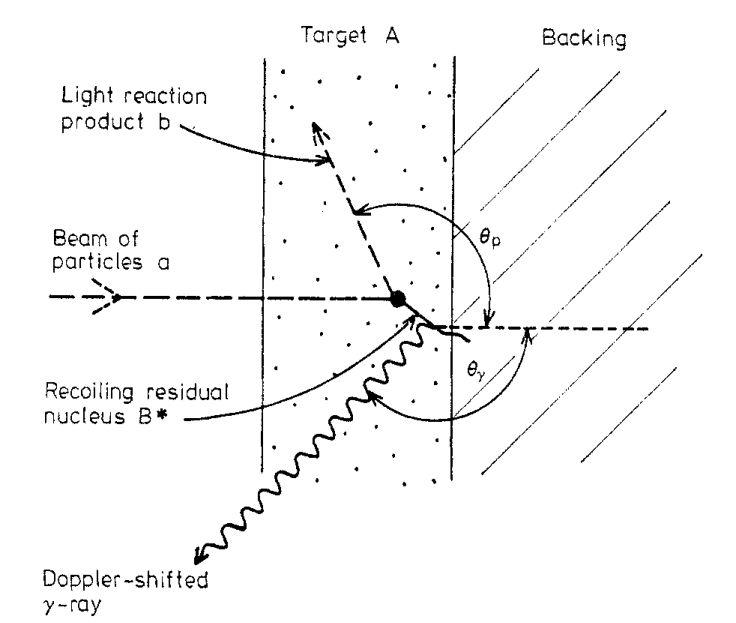
\includegraphics[width=0.7\textwidth]{js9-dsam.png}
\caption{Schéma metódy zoslabenia Dopplerovho posunu.}
\label{js9:img:dsam}
\end{figure}

Lúč nalietavajúcich častíc $a$ interaguje s jadrom $A$. Pri reakcii je emitovaný produkt $b$ a v materiály terčíku ostane excitované jadro $B^*$, ktorého polčas rozpadu chceme zmerať. Excitované jadro sa pohybuje v dôsledku spätného rázu s rýchlosťou $v_0$ a postupne v materiáli spomaľuje. Napokon vyžiari $\gamma$ žiarenie odpovedajúce strednej dobe života $\tau$ pri rýchlosti, ktorá klesla na hodnotu $\overline{v}$. Hodnotu $\overline{v}$ dokážeme zmerať tak, že zmeriame strednú energiu $\gamma$ žiarenia ako funkciu~$\theta_\gamma$:
\begin{equation}
\overline{E}=E_0\left(1+\frac{\overline{v}}{c}\cos \theta_\gamma\right)
\end{equation}

Následne určíme faktor zoslabenia $F=\frac{\overline{v}}{v_0}$. Ten porovnáme s teoretickou funkciou $F(\tau)$ a z nej tak dokážeme určiť strednú dobu života. Touto metódou sme schopní merať doby života $\sim 10^{-12}-10^{-15}\:\unit{s}$.

Túto metódu možno využiť pri viacerých experimentálnych usporiadaniach v závislosti od nalietavajúcich častíc:
\begin{enumerate}
\item Záchytové reakcie - jedná sa o záchyt častice (napr. protón alebo $\alpha$) v jadre a emitácii $\gamma$ žiarenia. V tomto prípade sa energia nalietavajúcej častice sčítava s energiou terčíkového jadra.

\item Reakcie budené ľahkými iónmi - experimentálne najbežnejší spôsob, akým obsadiť najnižšie stavy v jadre s využitím binárnych reakcií vybudených ľahkými projektilmi ako $p$, $d$, $t$, $\tau$ a $\alpha$ s energiami $3-20$ MeV. V týchto reakciách vzniká okrem excitovaného jadra aj jedna častica, ktorá je emitovaná ($n$, $p$, $d$ alebo $\alpha$).

\item Reakcie budené ťažkými iónmi - keď ťažký ión bombarduje terčík s energiou prevyšujúcou Coulombovskú bariéru, dochádza k vyparovaniu nukleónov. Pri reakcii $A(x$n, $y$p, $z\alpha )B^*$ dôjde k vypareniu $x$ neutrónov, $y$ protónov a $z$ $\alpha$-častíc v čase kratšom ako $10^{-15}\:\unit{s}$. To je doprevádzané mnohými dipólovými a kvadrupólovými prechodmi.

\item Inverzné reakcie - jedná sa o reakcie, kedy ľahké častice bombardujeme ťažkými, ako napr. pri skúmaní strednej doby života $^{13}$C bola pužitá reakcia $^2$H($^{12}$C, p)$^{13}$C.
\end{enumerate}

\subsection{Teórie zastavenia}

Brzdný čas excitovaného jadra v pevnom materiáli definuje časovú škálu pre merania metódou DSAM. Zoslabujúci faktor $F$ môžeme zapísať v tvare
\begin{equation}
F=\dfrac{\overline{v}}{v_0}=\dfrac{1}{v_0\tau}\int_0^{\infty}v(t)\exp(-t/\tau)\mathrm{d}t.
\label{js9:eq:attfact}
\end{equation}

Problémom však je, že nepoznáme, ako jadro spomaľuje, teda funkcia $v(t)$ je pre nás neznámou. Ako prvú aproximáciu môžeme uvažovať, že strata energie bude úmerná rýchlosti excitovaného jadra, teda $\mathrm{d}E/\mathrm{d}x \propto v$. Táto podmienka sa totiž ukazuje ako veľmi dobrá aproximácia pre brzdné procesy elektrónov v materiáli.

Túto závislosť môžeme sformulovať do tvaru
\begin{equation}
v(t)=v_0\exp(-t/\alpha),
\end{equation}
kde $\alpha$ je charakteristická konštanta materiálu opisujúca brzdný čas. Dosadením tejto aproximácie do vzťahu (\ref{js9:eq:attfact}), dostaneme výraz pre zoslabujúci faktor
\begin{equation}
F=\dfrac{1}{1+\tau/\alpha}.
\end{equation}

Tvar $\gamma$ spektrálnej čiary však tiež dokáže priniesť informáciu o dobe života. Rovniu (\ref{js9:eq:attfact}) preto môžeme zapísať do tvaru
\begin{equation}
F=\dfrac{1}{v_0}\dfrac{\int_0^{v_0}v\frac{\mathrm{d}N(v)}{\mathrm{d}v}\mathrm{d}v}{\int_0^{v_0}\frac{\mathrm{d}N(v)}{\mathrm{d}v}\mathrm{d}v},
\end{equation}
kde $N(v)$ je počet jadier, ktoré sa rozpadnú pri rýchlosti $v$. Keďže vieme, že 
\begin{equation}
\mathrm{d}N(t)=\frac{1}{\tau}e^{-t/\tau}\mathrm{d}t
\end{equation}
a navyše poznáme funkciu $v(t)$, môžeme si ľahko dopočítať závislosť $N$ na rýchlosti:
\begin{equation}
\mathrm{d}N(v)=\dfrac{\alpha}{v\tau}\left(\dfrac{v}{v_0}\right)^{\alpha/\tau}\mathrm{d}v.
\end{equation}

\subsection{Metóda vzdialenosti doletu spätného rázu}

Ďalšou metódou je metóda vzdialenosti doletu spätného rázu\footnote{angl. Recoil distance method (RDM)}.

My môžeme jadro zastaviť počas jeho letu, a to tak, že mu vo vzdialenosti $d=vt_0$ do cesty postavíme zachytávajúcu fóliu, prezývanú piest (plunger). Tie jadrá, ktoré dorazia na fóliu v excitovanom stave vyžiaria pri zastavené neposunutú $\gamma$-linku, zatiaľ čo tie jadrá, ktoré sa rozpadli skôr, vykazujú Dopplerovský posun. Celý proces je znázornený na obr. \ref{js9:img:rdm}.

\begin{figure}[h!]
\centering
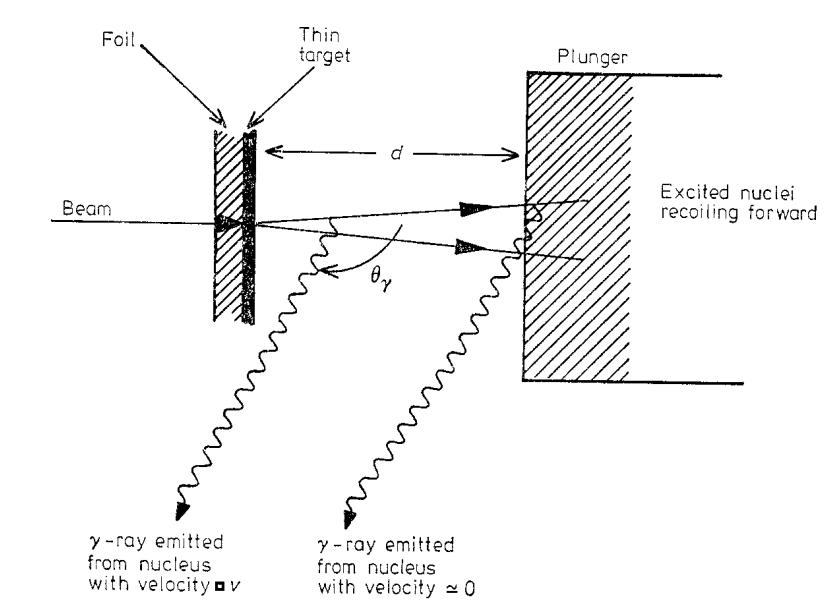
\includegraphics[width=0.7\textwidth]{js9-rdm.png}
\caption{Schéma metódy vzdialenosti doletu spätného rázu.}
\label{js9:img:rdm}
\end{figure}


Pomer intenzít $\gamma$ žiarenia vyžiareného jadrami počas pohybu a zastavenými jadrami je 
\begin{equation}
R(d)=\dfrac{S_\gamma^Z}{S_\gamma^Z+S_\gamma^P},
\end{equation} 
kde $S_\gamma^Z$ je intenzita vyžiarená zastavenými atómami a $S_\gamma^P$ intenzita vyžiarená atómami počas pohybu. Obe intenzity vypočítame ako
\begin{subequations}
\begin{equation}
S_\gamma^P=S(0)\int_0^{t_0}e^{-\frac{t}{\tau}}\mathrm{d}t
\end{equation}
\begin{equation}
S_\gamma^Z=S(0)\int_{t_0}^\infty e^{-\frac{t}{\tau}}\mathrm{d}t
\end{equation}
\end{subequations}

Keď si nakreslíme pomer týchto dvoch intenzít ako funkciu vzdialenosti $d$, môžeme veľmi ľahko určiť polčas rozpadu excitovaného stavu. Touto metódou je merateľná oblasť dôb života $\tau\sim 10^{-8}-10^{-12}\:\unit{s}$. Bežné hodnoty $d$ sú v rozmedzí $1-0,01\:\unit{mm}$, hrúbka terča $0,7-1,5\:\unit{\mu m}$, hrúbka fólie $5-10\:\unit{\mu m}$, pričom fólia je väčšinou z Au, Ta alebo Bi. 



\end{document}